% ===========================================
% Template for ICMC-NYCEMF 2019 (version2)
% adapted from earlier LaTeX paper templates for the ICMC, SMC, etc...
% ===========================================

\documentclass{article}
\usepackage{icmc2019template}
\usepackage{times}
\usepackage{ifpdf}
\usepackage{soul}
\usepackage[english]{babel}
%\usepackage{cite}


\long\def\markk#1{{\color{red}{\bf Mark: }{\small [#1]}}}
\long\def\samm#1{{\color{blue}{\bf Sam: }{\small [#1]}}}

\usepackage{flushend}


%%%%%%%%%%%%%%%%%%%%%%%% Some useful packages %%%%%%%%%%%%%%%%%%%%%%%%%%%%%%%
%%%%%%%%%%%%%%%%%%%%%%%% See related documentation %%%%%%%%%%%%%%%%%%%%%%%%%%
%\usepackage{amsmath} % popular packages from Am. Math. Soc. Please use the 
%\usepackage{amssymb} % related math environments (split, subequation, cases,
%\usepackage{amsfonts}% multline, etc.)
%\usepackage{bm}      % Bold Math package, defines the command \bf{}
%\usepackage{paralist}% extended list environments
%%subfig.sty is the modern replacement for subfigure.sty. However, subfig.sty 
%%requires and automatically loads caption.sty which overrides class handling 
%%of captions. To prevent this problem, preload caption.sty with caption=false 
%\usepackage[caption=false]{caption}
%\usepackage[font=footnotesize]{subfig}

% ====================================================
% ================ Define title and author names here ===============
% ====================================================
%user defined variables
\def\papertitle{Studio Report: Yale Open Music Initiative}
\def\firstauthor{Scott Petersen}
\def\secondauthor{Mark Santolucito}
\def\thirdauthor{Konrad Kaczmarek}

% adds the automatic
% Saves a lot of output space in PDF... after conversion with the distiller
% Delete if you cannot get PS fonts working on your system.

% pdf-tex settings: detect automatically if run by latex or pdflatex
\newif\ifpdf
\ifx\pdfoutput\relax
\else
   \ifcase\pdfoutput
      \pdffalse
   \else
      \pdftrue
  \fi
\fi

\ifpdf % compiling with pdflatex
  \usepackage[pdftex,
    pdftitle={\papertitle},
    pdfauthor={\firstauthor, \secondauthor, \thirdauthor},
    bookmarksnumbered, % use section numbers with bookmarks
    pdfstartview=XYZ % start with zoom=100% instead of full screen; 
                     % especially useful if working with a big screen :-)
   ]{hyperref}
  %\pdfcompresslevel=9

  \usepackage[pdftex]{graphicx}
  % declare the path(s) where your graphic files are and their extensions so 
  %you won't have to specify these with every instance of \includegraphics
  \graphicspath{{./figs/}}
  \DeclareGraphicsExtensions{.pdf,.jpeg,.png,.jpg}

  \usepackage[figure,table]{hypcap}

\else % compiling with latex
  \usepackage[dvips,
    bookmarksnumbered, % use section numbers with bookmarks
    pdfstartview=XYZ % start with zoom=100% instead of full screen
  ]{hyperref}  % hyperrefs are active in the pdf file after conversion

  \usepackage[dvips]{epsfig,graphicx}
  % declare the path(s) where your graphic files are and their extensions so 
  %you won't have to specify these with every instance of \includegraphics
  \graphicspath{{./figures/}}
  \DeclareGraphicsExtensions{.eps}

  \usepackage[figure,table]{hypcap}
\fi

%setup the hyperref package - make the links black without a surrounding frame
\hypersetup{
    colorlinks,%
    citecolor=black,%
    filecolor=black,%
    linkcolor=black,%
    urlcolor=black
}


% ====================================================
% ================ Title and author info starts here ===============
% ====================================================
% Title.
% ------
\title{\papertitle}

% Authors
% Please note that submissions are anonymous, therefore 
% authors' names should not be VISIBLE in your paper submission.
% They should only be included in the camera-ready version of accepted papers.
% uncomment and use the appropriate section (1, 2 or 3 authors)
%
% Single address
% To use with only one author or several with the same address
% ---------------
%\oneauthor
%   {\firstauthor} {Affiliation \\ %
%     {\tt \href{mailto:author@unt.edu}{author@unt.edu}}}

%Two addresses
% the default spacing is 1.5in, but this can be reduced to 0.5in or less, if needed
%--------------
% \twoauthors
%   {1.5in}
%   {\firstauthor} {Affiliation1 \\  %
%     {\tt \href{mailto:author1@unt.edu}{author1@unt.edu}}}
%   {\secondauthor} {Affiliation2 \\  %
%     {\tt \href{mailto:author2@unt.edu}{author2@unt.edu}}}

% Three addresses
% the default spacing is 0.5in, but this can be reduced to 0.3in or less, if needed
% --------------
 \threeauthors
   {0.2in}
   {\firstauthor} {Yale University\\ %
     {\tt \href{mailto:scott.petersen@yale.edu}{scott.petersen@yale.edu}}}
   {\secondauthor} {Yale University\\ %
     {\tt \href{mailto:mark.santolucito@yale.edu}{mark.santolucito@yale.edu}}}
   {\thirdauthor} {Yale University\\ %
     {\tt \href{mailto:konrad.kaczmarek@yale.edu}{konrad.kaczmarek@yale.edu}}}
% ===================================================
% =============== The document content starts here ===============
% ====================================================
\begin{document}
%
\capstartfalse
\maketitle
\capstarttrue
%
\begin{abstract}
This studio report describes the Yale Open Music Initiative (OMI) and the degree programs, spaces, events, and research surrounding the organization. OMI aims to foster a community of practice around the development and use of open source audio tools in the context of artistic expression. We give an overview of the key resources available to students, staff, and faculty for the exploration of creative computation and digitally-enabled music production.
\end{abstract}
%

\section{Introduction}

The \textit{Open Music Initiative (OMI)} at Yale is an experimental group that is inclusive to diverse student interests. Hosted within the Computer Science department, the OMI studio features a range of hardware and software focused on the creative use and development of open source technologies.

The Initiative is staffed by students and faculty of both the Computer Science and Music Departments. Highlights of OMI's activities include educational workshops for the university and broader creative community, as well as performances of faculty, staff, and student work. OMI also maintains ongoing research collaboration with other research labs in the Computer Science department at Yale.



\section{Degree Programs}

The OMI studio at Yale plays a part of the larger community of computation and the arts in the \textit{Creative Consilience (C2)} of Computing and the Arts program. The C2 program encompasses computer music studies and promotes the interaction and collaboration between the visual and performing arts (architecture, art, history of art, and theater studies), computer science, and information technology. The goal of C2 is to act as a leader in the space of computational arts and provide new and unique opportunities in computer science research and education.

Within the C2 program, Yale offers a Bachelor's degree in \textit{Computing and the Arts (CPAR)}, as well as specialized tracks in the graduate program for Master's and Doctoral students. Course offerings specific to computer music include \textit{Twenty-First Century Electronic and Computer Music Techniques}, \textit{Computer Music: Algorithmic and Heuristic Composition}, \textit{Computer Music: Sound Representation and Synthesis}, \textit{Fundamentals of Music Technology}, and \textit{Laptop Ensembles: Study and Performance}.



\section{Creative Spaces}

Yale boasts a number of spaces with diverse technological audio tools and acoustic infrastructure to support the creation of new electronic and computer music.

\begin{figure}[h]
    \centering
    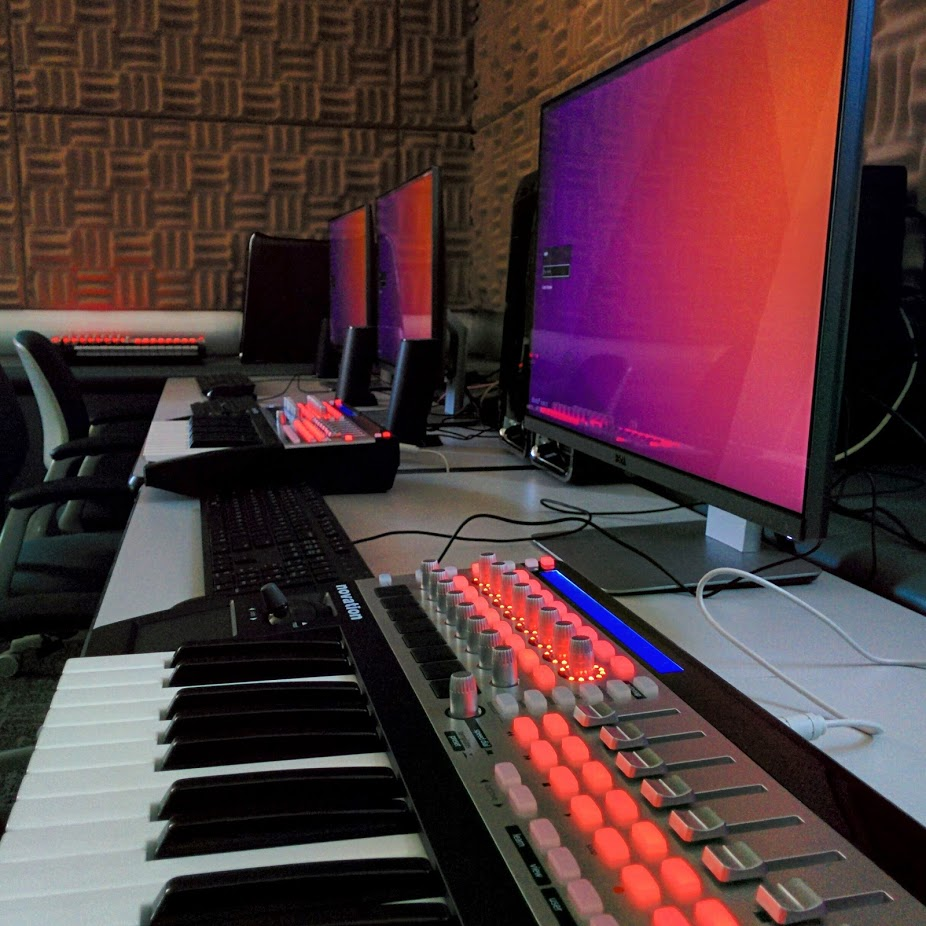
\includegraphics[width=0.85\columnwidth]{figs/euterpeastudio.png}
    \caption{The studio in AKW123}
    \label{fig:AKW123}
\end{figure}

\subsection{AKW 123}
OMI is based in the AKW 123 space in the Computer Science building. It is used to teach classes, conduct research, and host workshops and reading groups. The studio features desktop and mobile workstations for electroacoustic and new media composition built on open source synthesis and production toolchains. All workstations run a custom operating system consisting of a base Gnu-Linux OS, currently KDE Neon/Ubuntu, and a series of overlays and configurations to provide a low-latency environment with hundreds of software packages including DAWs, domain-specific audio programming languages such as SuperCollider, and a rich DSP and synthesis plugin collection. All lab machines can access the OMI server which, among other things, provides access to terabytes of sound samples.

The studio is equipped with a wide range of hardware including; digital and analog audio mixers and interfaces, 20 portable midi keyboards and miscellaneous MIDI and OSC controllers, built-in video projection, various studio microphones, field recording devices, electronic performance interfaces such as an EWI controller and a Yamaha AvantGrand N3 MIDI piano, game controllers, LEAP motion sensors, VR headsets (Oculus Rift and HTC Vive), and Microsoft Kinects. The studio also manages a collection of analog synthesizers, including a Novation Peak, a Moog Werkstatt, a microKORG Vocoder, and a Behringer Deepmind12. These are used in OMI's ``synth jams'', as well as for student projects. The space also supplies hardware components such as Arduinos, Bela Boards, and Raspberry Pis, as well as custom built hardware interfaces like the OMIPOD~\cite{omipod}. All hardware is made available to faculty and students for their own creative practice and research. 

\subsection{Center for Collaborative Arts and Media}

Additionally, OMI benefits from the rich ecosystem for computational arts at Yale. The Center for Collaborative Arts and Media (CCAM) is the central hub for C2-related activities. The center provides physical resources such as an audio-visual post-production suite and an 8-channel, reconfigurable transdisciplinary performance space equipped with a 32 camera motion capture system. The CCAM also provides human resources in the form of workshops and lectures by visiting artists and intellectuals, as well as those from the Yale community. Collaboration is at the heart of the center which provides ample opportunities for students and faculty to work together to workshop, research and produce creative work at the intersection of the sciences, arts and technology.

\subsection{Yale Music Technology Labs}

The Department of Music houses the Yale Music Technology Labs (YalMusT) which are comprised of two teaching labs, a small post-production studio and an advanced audio technology classroom. Both labs have surround-sound systems and the studio boasts a specially calibrated Genelec monitoring system. Further details on these spaces can be found online\footnote{\url{https://yalmust.yale.edu/}}.

\subsection{Residential College Studios}

The residential college system at Yale boasts five production studios that support audio recording, editing, and production. Each facility features a different set of equipment to expose students to a variety of studio environments. Furthermore, all studios are managed by student volunteers. Further details on these spaces can be found online\footnote{\url{https://up.yalecollege.yale.edu/production-resources/music-production-facilities}}.



\section{Events}

\begin{figure}[!h]
    \centering
    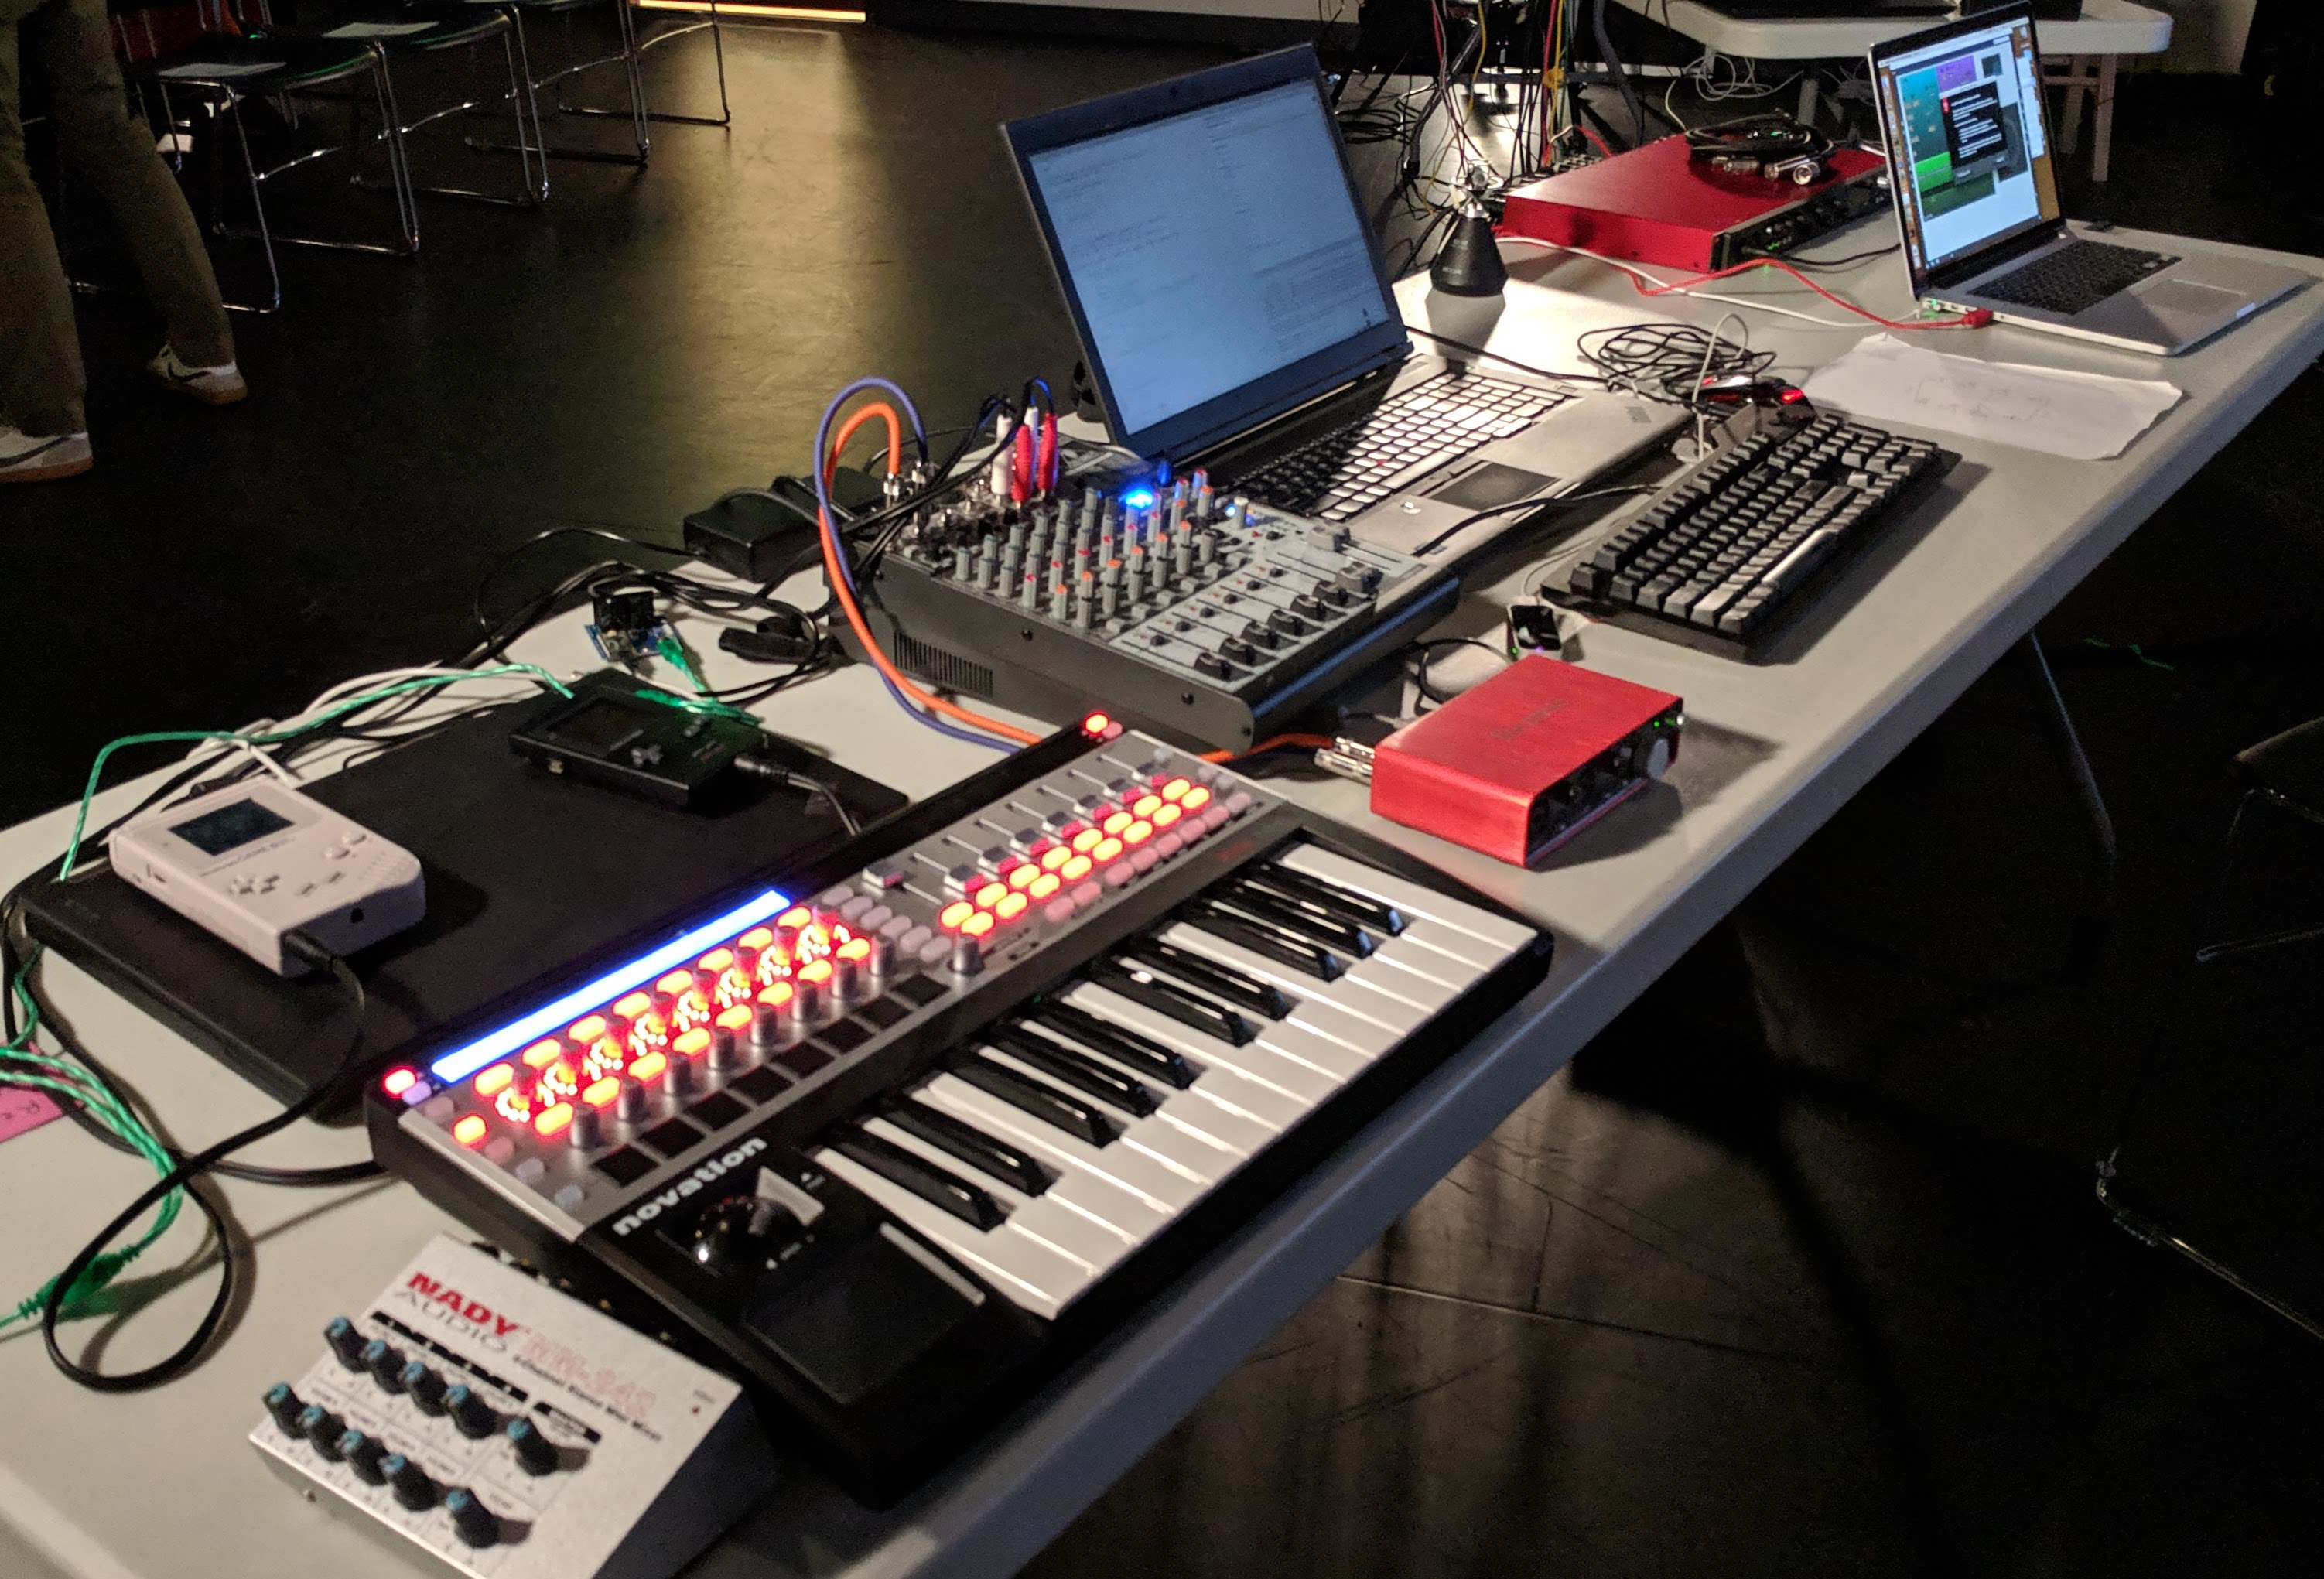
\includegraphics[width=0.85\columnwidth]{figs/concert.jpg}
    \caption{OMI using the CCAM space for a concert}
    \label{fig:concert}
\end{figure}

The OMI membership designs and coordinates a series of workshops that are offered over the course of the academic year at both the introductory and advanced level. Attendees typically represent a broad cross-section of schools and departments at Yale as well as local artists from the community. In the workshops, OMI members introduce relevant concepts and technologies in topics. In the fall of 2018, topics included: building an LM386 amplifier circuit, basic theory of DSP and DSP programming in JUCE~\cite{juce}, hacking ``found'' hardware, and an introduction to Arduino and sensor networks.


 
\begin{figure}
    \centering
    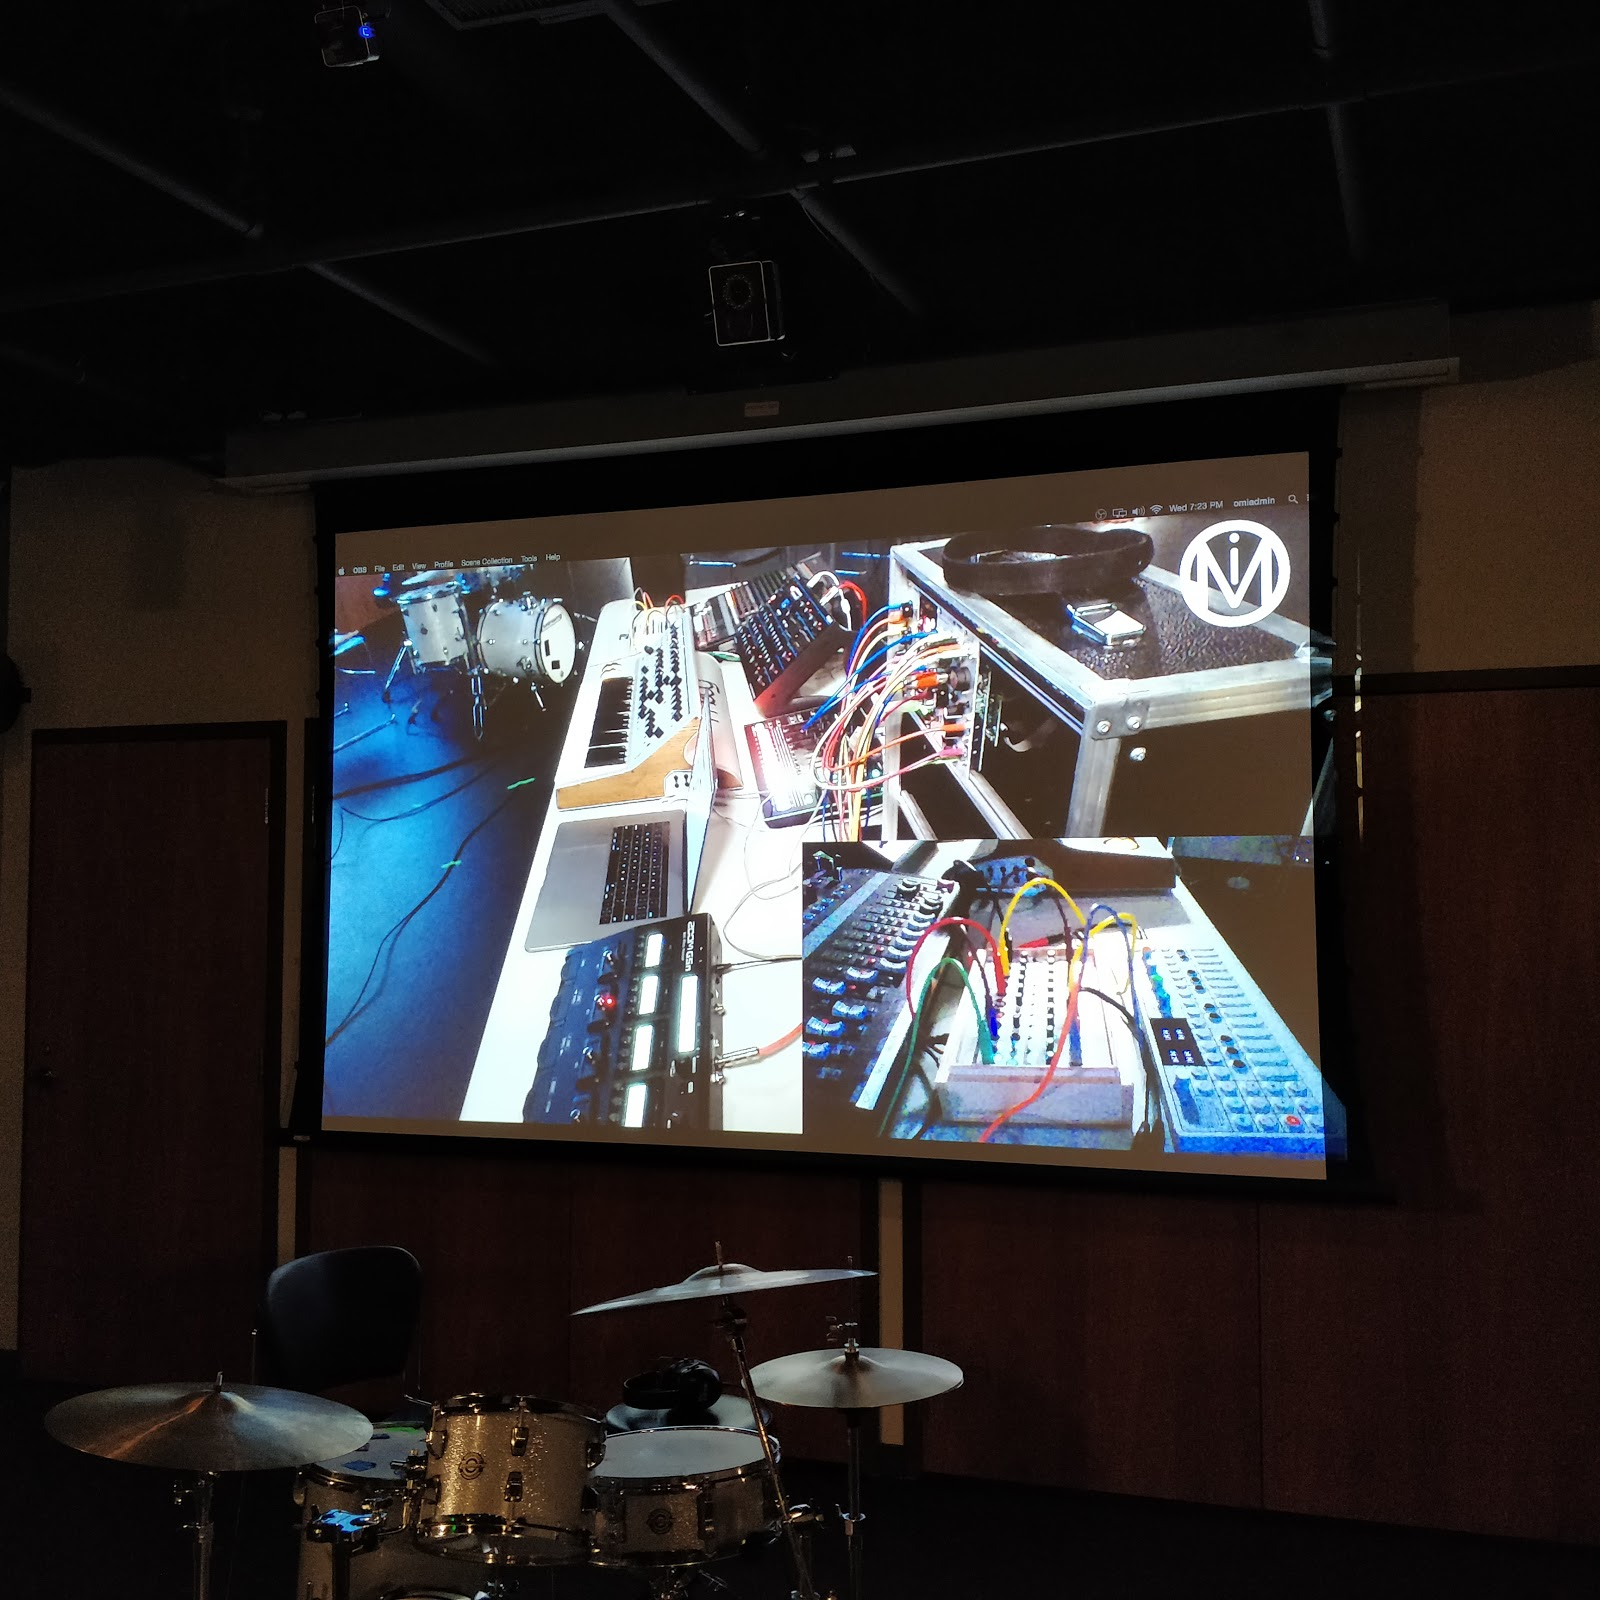
\includegraphics[width=0.85\columnwidth]{figs/concert2.jpg}
    \caption{OMI's end of semester concert}
    \label{fig:concert}
\end{figure}
 
In December 2018, OMI hosted a computer music concert showcasing work from students and faculty in the CCAM. The concert featured live electronics improvisation using analog and digital synthesizers, live coding, performances with interactive processing, and pieces utilizing eight-channel sound spatialization. A selection of the hardware used for this concert is shown in Fig.~\ref{fig:concert}.



\section{Research}

An important aspect of OMI is outreach and community involvement in our research. As an example, in September 2017, OMI ran a workshop in the CCAM that delved into the internal design of the OMIPOD, OMI's custom-made wireless musical instrument. The OMIPOD uses embedded hardware to relay information from different sensors (light, touch, tilt) over wi-fi to any computer on the Yale network.  In the interactive workshop participants experimented with the OMIPOD and learned about the hardware configuration, sensors and software necessary to program the device.

Undergraduate involvement in research is also a priority for OMI. A recent OMI project focused on the topic of Digital Signal Processing Programming by Example (DSP-PBE)~\cite{SantolucitoFARM}. DSP-PBE is a paradigm in which users specify input and output wave files, and a tool automatically synthesizes a program that transforms the input to the output. This work was completed as part of a funded summer undergraduate research internship of one student, as well as another student's undergraduate thesis. OMI is continuing this work with more undergraduates.



\section{Moving forward}

OMI will continue to support the many facets of computer music at Yale through weekly workshops, reading groups and through associated research projects. Specifically, we will focus on developing low-level DSP on Bela boards and DSP development over cloud computation frameworks. OMI will also continue its biannual concert series to provide faculty and students a regular, ongoing venue for their creative work. OMI also looks to foster inter-track collaboration within the C2 program to find new applications of computer music in other artistic domains. Additional information about OMI can be found at \url{https://omi.yale.edu}.


\flushend

\begin{acknowledgments}
This research sponsored in part by NSF grants CCF-1302327, CCF-1553168, CCF-1715387.
\end{acknowledgments} 

%%%%%%%%%%%%%%%%%%%%%%%%%%%%%%%%%%%%%%%%%%%%%%%%%%%%%%%%%%%%%%%%%%%%%%%%%%%%%
%bibliography here
\bibliography{biblio}

\flushend

\end{document}
